% -*- root: Main.tex -*-
\section{Non-parametric Bayesian Inference}
\textbf{BI for multivariate Gaussian: } $p(x^*|X) = \int p(x^*|\theta)p(\theta|X)d\theta = \mathbb{E}_{\theta \sim p(\cdot | X)}[p(x^*|\theta)] \approx \frac{1}{M}\sum_t p(x^*|\theta^{(t)})$ where $\theta^{(t)}\sim p(\cdot | X)$; $\mu \sim \mathcal{N}(m_0, V_0), \Sigma \sim IW(S_0, v_0) \Rightarrow \mu | \Sigma, X \sim \mathcal{N}(m_p, V_p), \Sigma | \mu, X \sim IW(S_p, v_p)$ Gibbs sampling: For semi-conjugate priors, iteratively resample acc. to tractable cond. dist. n times. The update does not need to be in exact order for l-dim and first M samples are discarded. \\
\textbf{BI for GMM: } Dirichlet distribution (DP) on $\pi$: $Dir(\pi|\alpha) = \frac{\Gamma(\sum_i \alpha_i)}{\prod_i \Gamma(\alpha_i)} \prod_i \pi_i^{\alpha_i - 1}, \sum_i \pi_i = 1$ \\
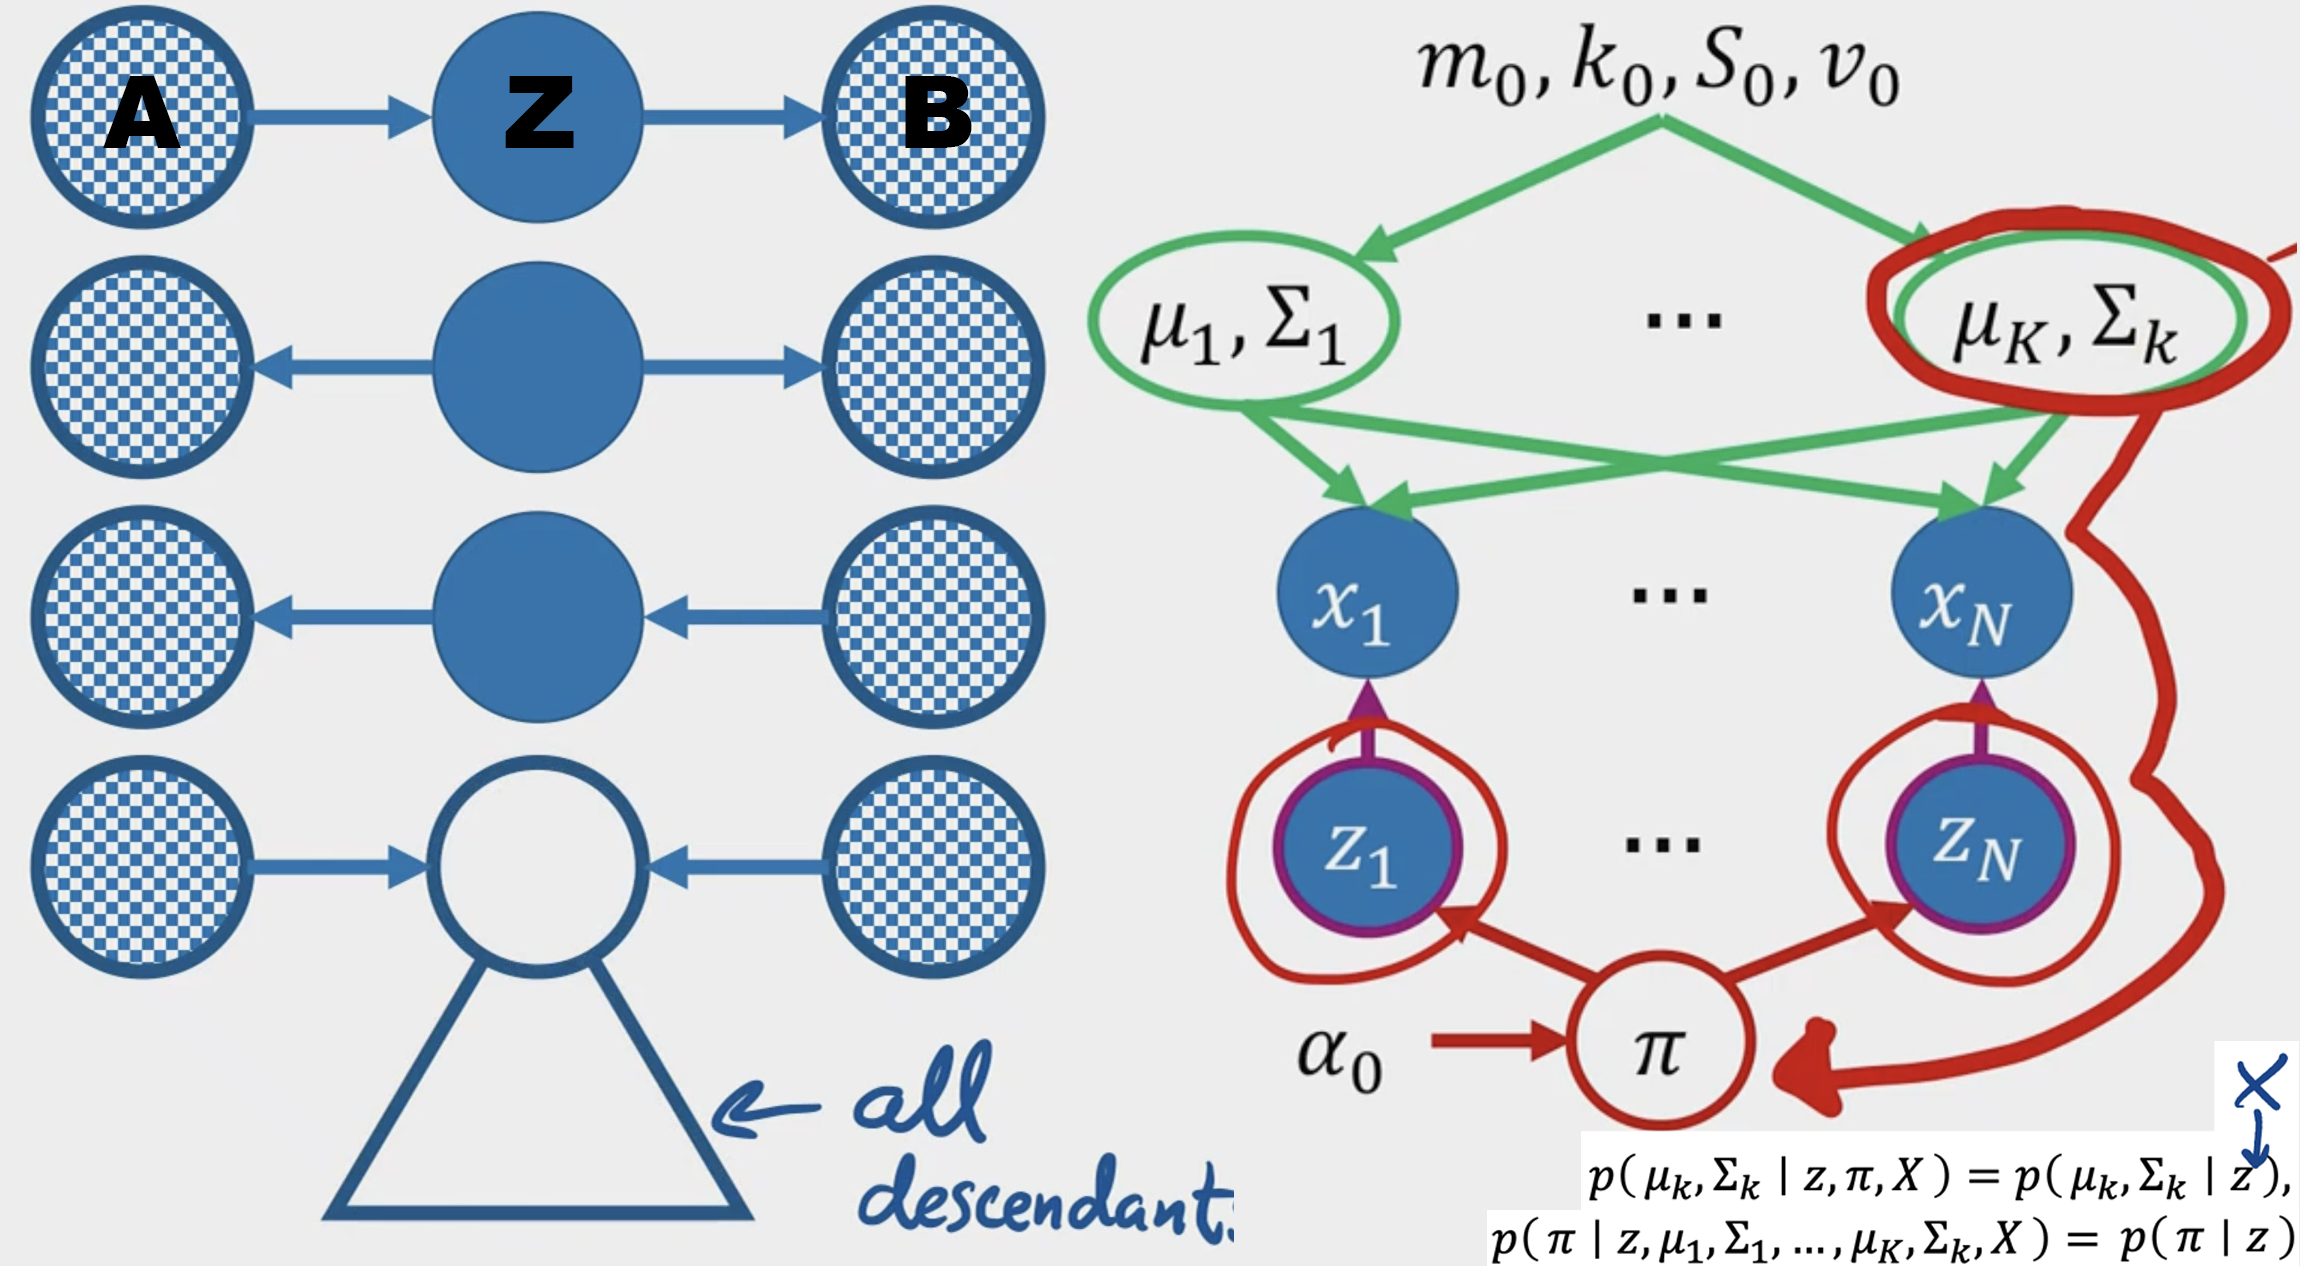
\includegraphics[scale=0.125]{d-separation.png}\\
If every path from variable A to B is blocked by d-separation Z, then A and B are independent conditioned on Z.\\
Collapsed Gibbs sampling: first sample z: $p(z_i = k | z_{-i} = \zeta, X) \propto p(z_i = k | z_{-i} = \zeta)p(X|z_i=k, z_{-i}=\zeta) \propto p(z_i = k | z_{-i} = \zeta)p(x_i|X_{-i}, z_i=k, z_{-i}=\zeta)p(X_{-i}|z_i=k, z_{-i}=\zeta) \propto p(z_i = k | z_{-i} = \zeta)p(x_i | \{x_j: j \leq N_{i \neq j}, z_j = k\})const$; \\
Rao-Blackwellization:
% $\mathbb{E}_{\theta, Z}[f(\theta, Z) | Z] \approx \frac{1}{M}\sum_i \mathbb{E}_{\theta}[f(\theta, z^{(i)}]$, $ z^{(i)}\sim p_z \approx \frac{1}{M}\sum_i f(\theta^{(i)}, z^{(i)})$, $\theta^{(i)}\sim p_{\theta}(\cdot | z^{(i)})$; 
$Var_Z[\mathbb{E}_{\theta}[f(\theta, Z)|Z]] = \mathbb{E}_Z[(\mathbb{E}_{\theta, Z}[f(\theta, Z)] - \mathbb{E}_{\theta'}[f(\theta', Z)])^2] = \mathbb{E}_Z[(\mathbb{E}_{\theta'}[\mathbb{E}_{\theta, Z}[f(\theta, Z)] - f(\theta', Z)])] \leq \mathbb{E}_Z[\mathbb{E}_{\theta'}[(\mathbb{E}_{\theta, Z}[f(\theta, Z)] - f(\theta', Z))^2]] = \mathbb{E}_{Z, \theta'}[(\mathbb{E}_{\theta, Z}[f(\theta, Z)] - f(\theta', Z))^2] = Var_{\theta', Z}[f(\theta', Z)]$ \\
\textbf{BI for non-parametric GMMs: }
% Prior: $\mu_k, \Sigma_k \sim NIW(...), \pi \sim GEM(\alpha), \alpha > 0$; 
Sampling prior: 1) Draw $\pi$ from $GEM(\alpha)$ with Stick-breaking Process: $\pi_1 = \beta_1 \sim Beta(1, \alpha)$, $\pi_{i, i\geq 2} = \prod_{j < i}(1-\beta_j)\beta_i$;
2) Chinese Restaurant Process (metaphor of DP, draw z directly): \\
$p(z_n=k) = $ \begin{cases}
      n_k/(\alpha+n-1), \text{for existing k} \\
      \alpha/(\alpha+n-1), \text{for leftmost empty k}
    \end{cases} \\
$z_1,...,z_n$ are not independent but exchangable. Proof: $p(z_1=k_1, ..., z_n = k_n) = \prod_i p(z_i=k_i|z_1=k_1, ..., z_n=k_n) = \prod_i \frac{f(\alpha, k_i)}{\alpha+i-1} = \prod_i\frac{f(\alpha, k_{\pi^{-1}(i)}}{\alpha+i-1} = p(z_{\pi(1)} = k_1,...,z_{\pi(n)} = k_n)$;
% 3) Dirichlet Process \\
% $(G(T_1), ..., G(T_m)) \sim Dir(\alphaH(T_1), ..., \alphaH(T_m))$ \\
Asymptotics of the expected \# of distinct samples drawn / expected \# of occupied tables in CRP: $S(n) = \sum_k \frac{\alpha}{\alpha+k-1} \geq I(n) = \int_{1}^{n+1}\frac{\alpha}{\alpha+x-1}dx = \alpha(ln(\frac{\alpha+n}{\alpha}))$
\\
DeFinetti’s Theorem: any exchangeable distribution admits a mixture model, $p(X_1 = x_1, ..., X_n = x_n) = \int \prod_i p(x_i|\theta)p(\theta)d\theta$
